%%%%%%%%%%%%%%%%%%%%%%%%%%%%%%%%%%%%%%%%%%%%%%%%%%%%%%%%%%%%%%%%%%
%%%%%%%% ICML 2016 EXAMPLE LATEX SUBMISSION FILE %%%%%%%%%%%%%%%%%
%%%%%%%%%%%%%%%%%%%%%%%%%%%%%%%%%%%%%%%%%%%%%%%%%%%%%%%%%%%%%%%%%%

% Use the following line _only_ if you're still using LaTeX 2.09.
%\documentstyle[icml2016,epsf,natbib]{article}
% If you rely on Latex2e packages, like most moden people use this:
\documentclass{article}

% use Times
\usepackage{times}
% For figures
\usepackage{graphicx} % more modern
%\usepackage{epsfig} % less modern
\usepackage{subfigure} 

% For citations
\usepackage{natbib}

% For algorithms
\usepackage{algorithm}
\usepackage{algorithmic}

% As of 2011, we use the hyperref package to produce hyperlinks in the
% resulting PDF.  If this breaks your system, please commend out the
% following usepackage line and replace \usepackage{icml2016} with
% \usepackage[nohyperref]{icml2016} above.
\usepackage{hyperref}

% Packages hyperref and algorithmic misbehave sometimes.  We can fix
% this with the following command.
\newcommand{\theHalgorithm}{\arabic{algorithm}}

% Employ the following version of the ``usepackage'' statement for
% submitting the draft version of the paper for review.  This will set
% the note in the first column to ``Under review.  Do not distribute.''
\usepackage[accepted]{icml2016} 

% Employ this version of the ``usepackage'' statement after the paper has
% been accepted, when creating the final version.  This will set the
% note in the first column to ``Proceedings of the...''
%\usepackage[accepted]{icml2016}


% The \icmltitle you define below is probably too long as a header.
% Therefore, a short form for the running title is supplied here:
\icmltitlerunning{Middle report for Advanced Machine Learning project}

\begin{document} 
\twocolumn[
\icmltitle{Mid-report for \\ 
           Advanced Machine Learning project}
% It is OKAY to include author information, even for blind
% submissions: the style file will automatically remove it for you
% unless you've provided the [accepted] option to the icml2016
% package.
\icmlauthor{Xiaoxiao CHEN}{xiaoxiao.chen@telecom-paristech.fr}
\icmlauthor{Yuxiang WANG}{yuxiang.wang@u-psud.fr}
\icmlauthor{Honglin LI}{hong-lin.li@u-psud.fr}

% You may provide any keywords that you 
% find helpful for describing your paper; these are used to populate 
% the "keywords" metadata in the PDF but will not be shown in the document
\icmlkeywords{boring formatting information, machine learning, ICML}

\vskip 0.3in
]

\begin{abstract} 
The purpose of this middle report of the project is to present the problem we plan to solve and the progress of the project and also the problems we meet. The whole report will be divided into 5 parts: (1) Introduction: present the problem and our plan; (2) Recommendation system: present the data set and the specific methods we are using; (3) Evaluation: the evaluation metrics of this challenge; (4) Discussion and perspectives: all the problems we meet so far and their potential solutions; (5) Conclusion: the work need to be done and the future plan of the project.
\end{abstract} 


\section{Introduction}
The Million Song Dataset Challenge aims at being the best possible offline evaluation of a music recommendation system. Any type of algorithm can be used: collaborative filtering, content-based methods, web crawling,etc. By relying on the Million Song Dataset, the data for the competition is completely open: almost everything is known and possibly available.

The specific task can be described briefly. The data we have is: 1) the full listening history for 1M users which is the original data set, 2) half of the listening history for 110K users, and another missing half should be predicted and compared to the results. 

The most straightforward approach to this task is pure collaborative filtering, but there is a wealth of information available to the data scientist through the Million Song Dataset. In  other words, the content-based methods have various possibilities and we have plenty of things to experiment which might bring us some surprising results.

For so far, we have met several problems in both theoretical aspect and engineering aspect. We will discuss the baseline method we have set and the potentials of other better methods. The different forms of evaluation metrics will also be discussed.
\section{Recommendation system}
Recommender systems or recommendation systems are a subclass of information filtering system that seek to predict the "rating" or "preference" that a user would give to an item. Recommender systems have become increasingly popular in recent years, and are utilized in a variety of areas including movies, music, news, books, research articles, search queries, social tags, and products in general. There are also recommender systems for experts, collaborators, jokes, restaurants, garments, financial services, life insurance, romantic partners (online dating), and Twitter pages.

\subsection{Challenge problem}
In our context, a music recommendation system need to be developed to predict the preferences of the existing users based on their listening history. The original data set consists of the listening history of 1M users, the challenge data is about 110K users. The data set is manually divided into train set and test set, each consists of half of the listening history.

Our mission is to use the train set to develop a model to do the prediction of the test set. The kaggle site used \emph{Root mean square error} as their evaluation metric, but we are able to set our own metrics since the kaggle competition is already closed. According to the evaluation metric, the problem can be also regarded as classification problem or regression problem. The details will be discussed in section 3.
\subsection{Data Analysis}
There are four files available at kaggle site:
\begin{itemize}
\item  {kaggle\_visible\_evaluation\_triplets.txt} - this is the core data: triplets( \emph{user,song,play count} ). The play count are generally considered equal as the rating of different songs from the user. The more a song played by a user, the more preference showed by the user on this song.
\item {kaggle\_users.txt} - this is the canonical list of user identifiers, which must be used to sort the predictions.
\item {kaggle\_songs.txt} - this is the canonical list of songs, which contains all song IDs from the training data and the test data.
\item {taste\_profile\_song\_to\_tracks.txt} - this file includes the information of the corresponding track for each song, by this information we can extract more information(artist, release year) from the external sources.
\end{itemize}

Since the original data comes from kaggle site and the submission channel is already closed, we are not able to evaluate our results on-line. In order to solve this problem, which means find a reference values for our prediction results, we managed to find the evaluation results from the site  \url{http://labrosa.ee.columbia.edu/millionsong/challenge#data1}. The visible part can be reconstructed as train data, and the hidden part can be used directly as evaluation data.

\begin{figure}[ht]
\vskip 0.2in
\begin{center}
\centerline{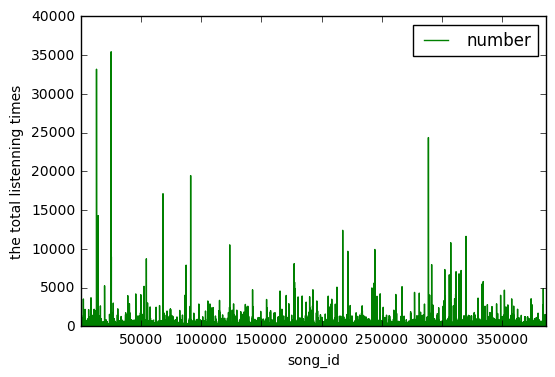
\includegraphics[width=\columnwidth]{sum111}}
\caption{the distribution of the total number of each song in the list}
\label{fig:total number}
\end{center}
\vskip -0.2in
\end{figure} 
The figure ~\ref{fig:total number} show  the total listening number of each song in the list, it can be seen from the figure, the  disparity  between different song is huge.  The listening number of  some songs is very little even zero, but some of them are more than  30k listening times. In fact, the song more popular will be more probable to be recommended. So, we can recommend directly the most popular song to all users.

\label{data}
\begin{figure}[ht]
\vskip 0.2in
\begin{center}
\centerline{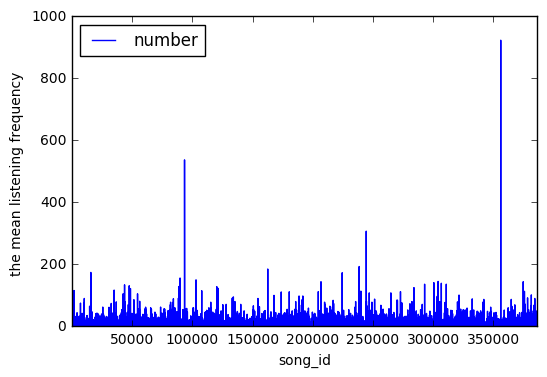
\includegraphics[width=\columnwidth]{mean_fre}}
\caption{The mean listening frequency for each song in the list}
\label{fig:mean_frequency}
\end{center}
\vskip -0.2in
\end{figure} 
The figure ~\ref{fig:mean_frequency} shows us some special information different from figure 1. This figure shows the  mean frequency of each song. In our natural mind, we think the song more popular will be listened more times for each person. In fact, it is not. Some popular song, it is just listened by many people, but each people will not take much time to repeat it, maybe it is not special but just popular. But for some special songs, maybe it is not so popular as the other, but it is special for some listener, maybe because its special style or its singer. So we can find that, for some special song, the fans of these song repeat more than 400 times. It is incredible that, if this song take 3 minutes, its fans take more than 20 hours to listen it.  As the result, we can recommend these special songs to those special listener, maybe based on the artist, maybe based on the style of the song etc.





\subsection{Methods}
Broadly speaking, recommender systems are based on one of two strategies. The \textbf{content filtering approach}~\ref{fig:content_filtering} creates a profile for each user or product to characterize its nature. For example, a song profile could include attributes regarding its genre, the artist, and so forth. User profiles might include demographic information or answers provided on a suitable questionnaire. The profiles allow programs to associate users with matching products. Of course, content-based strategies require gathering external information that might not be available or easy to collect.But in this case all the attributes of the songs are available on the web site \url{http://labrosa.ee.columbia.edu/millionsong/pages/example-track-description}. A trained music analyst finally scores each song based on hundreds of distinct musical characteristics. These attributes, or genes, capture not only a song’s musical identity but also many significant qualities that are relevant to understanding listeners’ musical preferences.

\begin{figure}[ht]
\vskip 0.2in
\begin{center}
\centerline{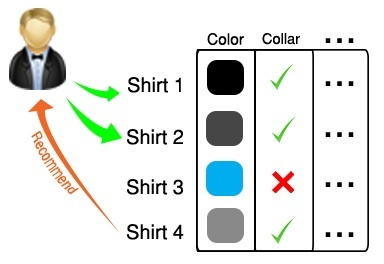
\includegraphics[width=\columnwidth]{content_based}}
\caption{Content Filtering approach}
\label{fig:content_filtering}
\end{center}
\vskip -0.2in
\end{figure}

An alternative to content filtering relies only on past user behavior. For example, previous transactions or product ratings without requiring the creation of explicit profiles. This approach is known as \textbf{collaborative filtering}~\ref{fig:cf}. Collaborative filtering analyzes relationships between users and interdependencies among products to identify new user-item associations. A major appeal of collaborative filtering is that it is domain free, yet it can address data aspects that are often elusive and difficult to profile using content filtering. While generally more accurate than content-based techniques, collaborative filtering suffers from what is called the cold start problem, due to its inability to address the system’s new products and users. In this aspect,content filtering is superior.

\begin{figure}[ht]
\vskip 0.2in
\begin{center}
\centerline{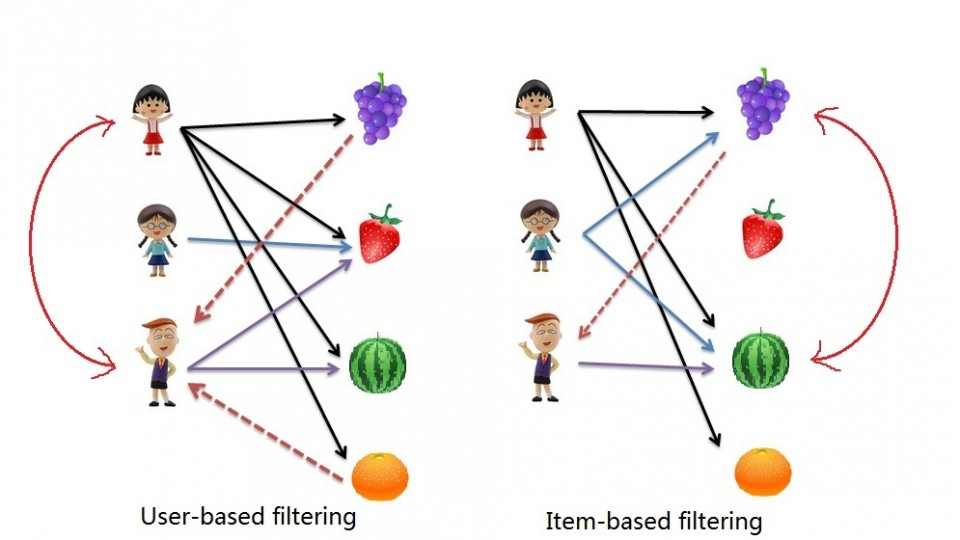
\includegraphics[width=\columnwidth]{collaborativeFiltering}}
\caption{Collaborative Filtering}
\label{fig:cf}
\end{center}
\vskip -0.2in
\end{figure}

The two primary areas of collaborative filtering are the neighborhood methods and latent factor models. Neighborhood methods are centered on computing the relationships between items or, alternatively, between users. The item-oriented approach evaluates a user’s preference for an item based on ratings of “neighboring” items by the same user. A product’s neighbors are other products that tend to get similar ratings when rated by the same user. 

\subsubsection{user-based with cosine similarity}
\begin{algorithm}[tb]
   \caption{User based with cosine similarity}
   \label{alg:example}
\begin{algorithmic}
   \STATE {\bfseries Input:} training\_matrix $M(m,n)$, prediction\_vector $y(1,n)$
   \STATE Calculate the similarity between training\_matrix and prediction\_vector
   \FOR{$row=1$ {\bfseries to} $m$}
   \STATE $sim(m_{row},y) = \frac{\sum^{n}_{i = 1}m_{i}*y{i}}{\|m_{row}\|_{2}*\|y\|_{2}}$
   \ENDFOR
   \STATE Recombine the similarity
   \FOR{$column=1$ {\bfseries to} $n$}
   \STATE $r_{col}=\frac{\sum_{i=1}^{m}sim(m_{i},y)*m_{i,col}}{\sum_{i=1}^{m} \|sim_{i}\|_{2}}$
   \ENDFOR
\end{algorithmic}
\end{algorithm}
We have tried the user-based with cosine similarity. known as vector-based similarity, we can use  cosine similarity to present the user action similarity. For example, if the user A like song 1,2,3, and user B also like song 1,2,3, it is reasonable that the user A is similar to user B. Naturally, if user A like  song 4, we can recommend it to user B.  In this algorithm, we calculate firstly the similarities between the candidate and all the  users, if the user  is  similar to the candidate,  the rating of the candidate will be more similar to this user.  In this algorithm, the similarity is treated as a weight to each user, and  the combination of all the user and their similarity will be the rating of the candidate.
After implementing the algorithm, We basically achieved a simple recommendation system with user-based. And we encountered some problems. Firstly, the size of the data is too big. When we translated the original data into a matrix, our memory was overloaded. In fact, we can not create a matrix with (110000,380000) which means the number of users and the number of songs. So for making the unit test for our algorithm, we selected the first 10 percents of data, which contains 840 users and 8087 songs.  So we think we should find some other methods, because this algorithm is not suitable for lager number of users. Secondly, it is  too bad for new user, because for a new user, we can not calculate the similarity . In other words, the similarity can not present the relation between old user and new user. However, this algorithm give us some ideas for recommendation system and return us an acceptable result.
\begin{figure}[ht]
\vskip 0.2in
\begin{center}
\centerline{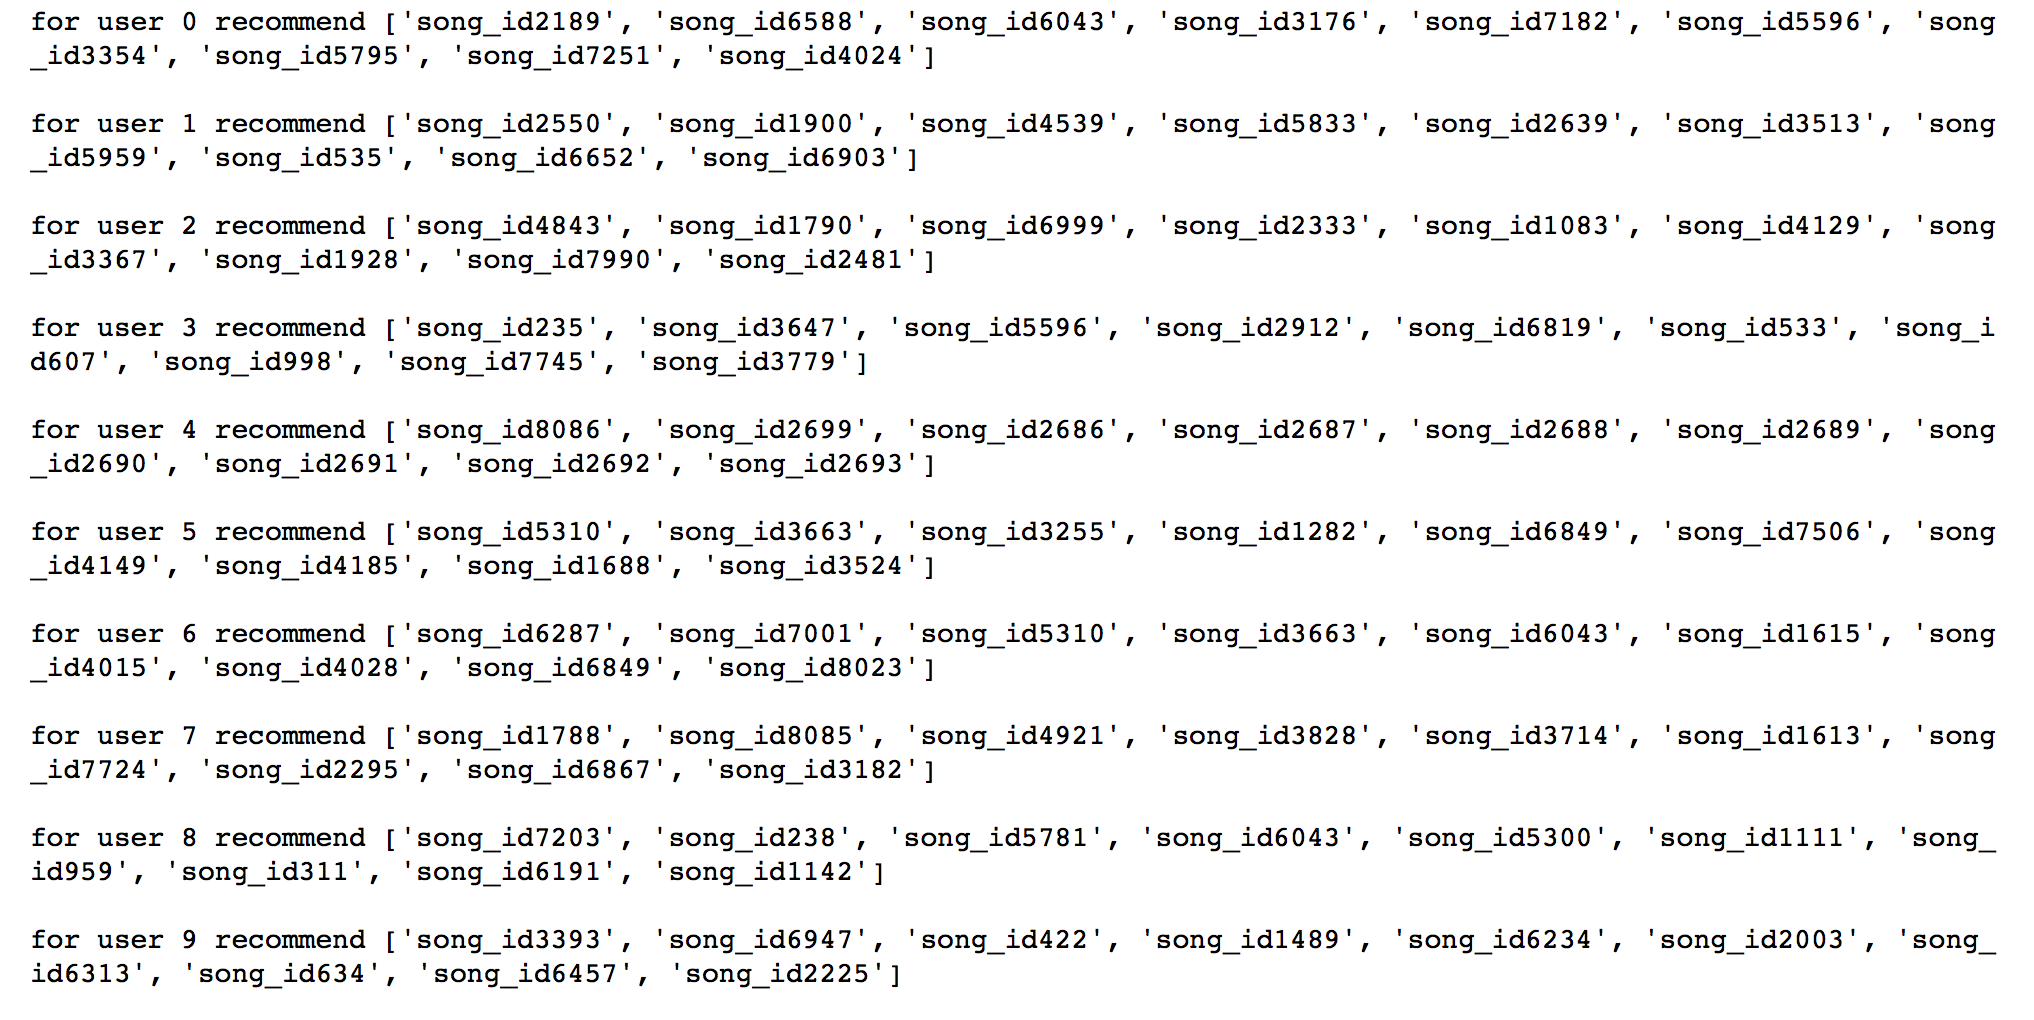
\includegraphics[width=\columnwidth]{test}}
\caption{The result of user-based with cosine similarity}
\label{fig:cf}
\end{center}
\vskip -0.2in
\end{figure}


\subsection{Baseline method}
As mentioned in the previous section, we can no longer evaluate our prediction result on-line, so we need to find a result as a standard baseline for reference. The challenge provides a \emph{getting started file} to help us get familiar with the data set and also its result can serve as a baseline to our model. The algorithm details are showed in Algorithm ~\ref{alg:baseline}. 

\begin{algorithm}[tb]
   \caption{Recommendation based on raw popularity}
   \label{alg:baseline}
\begin{algorithmic}
   \STATE {\bfseries Input:} triplets $(u_i,song_i,play\_discout_i)$, user\_id $u$,triplet size $m$,limited  size $k$
   \STATE Initialize $x = dict(song,count), r = dict(user,song list)$.
   \STATE Count the number of each song played in the train set and sort as the  
   \FOR{$i=1$ {\bfseries to} $m$}
   \STATE $x_i=x_i+1$
   \ENDFOR
   \STATE $x$ ordered descending order
   \STATE recommend the most popular songs to all the users
   \FOR{all users}
   \IF{$s$ from x and size $r<k$}
   \STATE $r.append(s)$
   \ENDIF
   \ENDFOR
\end{algorithmic}
\end{algorithm}

The system recommends the most popular songs among all the users to each user. They delete the song a specific user has already listened and recommend 500 new songs for each user. We can take a reference from the result, which shows a very basic way to recommend songs.
\section{Evaluation}
Evaluation is important in assessing the effectiveness of recommendation algorithms. The commonly used metrics are the mean squared error and root mean squared error.
Mean square error: \\
$MSE = \frac{1}{n}\sum_{i=1}^{n}(y_{i}^{*}-y_{i})^{2}$
\\
Root mean square error:\\
$RMSD = \sqrt[]{\frac{\sum_{i=1}^{n}(y_{i}^{*}-y_{i})^{2}}{n}}$

Another way to evaluate is to transform the final problem to a classification problem. According to the play count, we can divide the value into subsection as a class. But this form requires enormous workload of encoding. We will study its viability.

\section{Discussion and perspectives}
\subsection{problems}
we have encountered some problems in our project.
\begin{itemize}
\item  the size of data\\
the size of data is too large in this challenge. There are  110k users and more than 380k songs in the data. And the training set contain more than 1500k rows of records. We can not calculate directly by our computer, even just calculate the mean of each row, our computer was overloaded. 
\item  sparse data\\
The data is too sparse. There are many zeros in each row. In general, each user listens less than 1000 songs, but this size of song is 380K. The sparse date lead to  large error of prediction. For example, for the cosine similarity, more zeros means the similarity is less creditable. 
\item lack of information\\
From the data set, we just know the user listened a song. But we have not enough information about the  user and the song. It makes us too hard to improve our performance. So we think we need to find more information from other resource or other ways. For example, the lyrics of the song, the artist of the song etc. 
\item evaluation of performance\\
For this challenge, it is difficult to evaluate the performance. The recommendation system, it is different from the classification or regression problem, because there are so many ways to evaluate the performance. In general, we can use MSE and RMSD to evaluate the loss. But some times, we do not even know whether our prediction is suitable for the user, because we can not get the current feed-beck. We assume that we have a new method which is total different to the others, it make a new recommendation to a user, maybe it is a new and interesting subject to this user, but it is different type from user's habit. But in fact, we can not judge whether it is good for this user and we just know it is different to this user's habit. 
\end{itemize}
we would like to try some other methods in the following work.
\subsection{potential methods}
\begin{itemize}
\item Singular Value Decomposition:\\
For a matrix M, its SVD is the factorization of M into three constituent matrices such that $M = U\sum T^{T} $, $\sum$ is a diagonal matrix whose values $\theta_{i}$ are the singular values of the composition, and both U and T are orthogonal. After reading some papers and document, we find that Singular value decomposition can reduce the dimensionality of a dataset, and it can improve the accuracy of prediction.
\item Content-based method:\\
Basically, the use an item profile (i.e., a set of discrete attributes and features) characterizing the item within the system. The system creates a content-based profile of users based on a weighted vector of item features. The weights denote the importance of each feature to the user and can be computed from individually rated content vectors using a variety of techniques.

In our case, most of the fields about a specific track could be taken directly from the Echo Nest Analyze API. Some interesting attributes are listed below:
\begin{enumerate}
\item artist - many fans like to listen especially the music of certain artists
\item genre - rock and country has their own listener
\item tempo \& beats - rhythm is a significant character of certain genre of songs 
\item year - old music or new music
\end{enumerate}
Based on all these extra information, we have various possibilities to characterize each song and try to make a more predictive model.
\item Hybrid recommender systems:\\
Hybrid approaches can be implemented in several ways: by making content-based and collaborative-based predictions separately and then combining them; by adding content-based capabilities to a collaborative-based approach (and vice versa); or by unifying the approaches into one model. These methods can also be used to overcome some of the common problems in recommender systems such as cold start and the sparsity problem. We would like to study carefully the possibilities to integrate several models to reach a better performance.
\end{itemize}
\section{Conclusion}
In conclusion, we have finished our plan that we implemented our first version of recommendation system, and we got the result. Then,  after reading some document and discussing with each other, we found our problems and tried to find some ways to solve them. In the following work, we need to implement the  some new algorithms and try to  recombine them. 
\section{References}
[1] wikipedia about recommendation system\\$https://en.wikipedia.org/wiki/Recommender_system$

[2] M.D.Ekstrand, J.T.Riedl and J.A.Konstan\\
Collaborative Filtering Recommender Systems, P89-P101

[3] Website of  Mr.Antoine Cornuéjols \\$www.agroparistech.fr/ufr$-$info/membres/cornuejols/Teaching/Master$-$AIC/$

[4] Slides of course of stanford\\
$http://infolab.stanford.edu/~ullman/mmds/ch9.pdf$

[5] Slides of course of Mr. Xavier Amtriain\\
$http://fr.slideshare.net/xamat/recommender-systems-machine-learning-summer-school-2014-cmu$

% In the unusual situation where you want a paper to appear in the
% references without citing it in the main text, use \nocite

\nocite{langley00}

\bibliography{example_paper}
\bibliographystyle{icml2016}

\end{document} 


% This document was modified from the file originally made available by
% Pat Langley and Andrea Danyluk for ICML-2K. This version was
% created by Lise Getoor and Tobias Scheffer, it was slightly modified  
% from the 2010 version by Thorsten Joachims & Johannes Fuernkranz, 
% slightly modified from the 2009 version by Kiri Wagstaff and 
% Sam Roweis's 2008 version, which is slightly modified from 
% Prasad Tadepalli's 2007 version which is a lightly 
% changed version of the previous year's version by Andrew Moore, 
% which was in turn edited from those of Kristian Kersting and 
% Codrina Lauth. Alex Smola contributed to the algorithmic style files.  